% -*- latex -*-
%-----------------------------------------------------------------------
%;  Copyright (C) 2004
%;  Associated Universities, Inc. Washington DC, USA.
%;
%;  This program is free software; you can redistribute it and/or
%;  modify it under the terms of the GNU General Public License as
%;  published by the Free Software Foundation; either version 2 of
%;  the License, or (at your option) any later version.
%;
%;  This program is distributed in the hope that it will be useful,
%;  but WITHOUT ANY WARRANTY; without even the implied warranty of
%;  MERCHANTABILITY or FITNESS FOR A PARTICULAR PURPOSE.  See the
%;  GNU General Public License for more details.
%;
%;  You should have received a copy of the GNU General Public
%;  License along with this program; if not, write to the Free
%;  Software Foundation, Inc., 675 Massachusetts Ave, Cambridge,
%;  MA 02139, USA.
%;
%;  Correspondence concerning AIPS should be addressed as follows:
%;          Internet email: aipsmail@nrao.edu.
%;          Postal address: AIPS Project Office
%;                          National Radio Astronomy Observatory
%;                          520 Edgemont Road
%;                          Charlottesville, VA 22903-2475 USA
%-----------------------------------------------------------------------
%Body of final AIPSletter for 31 December 2003

\documentclass[twoside]{article}
\usepackage{graphics}

\newcommand{\AIPRELEASE}{December 31, 2003}
\newcommand{\AIPVOLUME}{Volume XXIII}
\newcommand{\AIPNUMBER}{Number 2}
\newcommand{\RELEASENAME}{{\tt 31DEC03}}
\newcommand{\OLDNAME}{{\tt 31DEC02}}
\newcommand{\NEWNAME}{{\tt 31DEC04}}

%macros and title page format for the \AIPS\ letter.
\input LET98.MAC

\newcommand{\MYSpace}{-11pt}

\normalstyle

\section{General developments in \AIPS}

\subsection{Spam and e-mail}

We receive on the order of 100 offers each day, many to enlarge
portions of daip's anatomy or to reduce the rest, to tranquilize
aipsmail while exciting some portions, to make money fast from home,
to get out of debt ``legally,'' to cheat producers of DVDs and other
entertainment, to add to our PhD degrees presumably to avail ourselves
of the many government grant programs, and, of course, to help wealthy
widows and orphans in Africa. And then there are those that are
totally gibberish or in some unknown foreign language.  Please, if you
need to reach us via e-mail, put a subject line that will be obviously
concerned with AIPS installation or execution difficulties.  If you do
not hear from us in a few days, send the e-mail again with an improved
subject line.  We hit the ``d'' key all too rapidly these days.

\subsection{Current and future releases}

We now have formal \AIPS\ releases on an annual basis with binary
releases only for Solaris and Linux.  All architectures can do a full
installation from the source files.  The current release is called
\RELEASENAME\ and is now frozen.  If you took a development copy of
this version at some earlier date, you may use the ``Midnight Job''
(MNJ) to bring it up to date.  You need to run a MNJ only once in 2004
to convert your copy of \RELEASENAME\ into the now frozen version.
This \Aipsletter\ is intended to advise you of developments in this
release.

We have begun a new version, called \NEWNAME, which is now under
development by the \AIPS\ Group.  You may fetch and install
a complete copy of this version at any time.  Having fetched \NEWNAME,
you may update your installation whenever you want by running the MNJ
which uses transaction files to copy and compile the code selectively
based on the code changes and compilations we have done.  We expect
users to take the source-only version of \NEWNAME\ \AIPS\ over the
Internet (via \emph{anonymous} ftp).

The MNJ has been changed.  The secure shell, with all its fragile
complexities, is no longer required.  Instead {\tt mnj.aoc.nrao.edu}
will serve up \AIPS\ incrementally --- or as a whole --- using the
Unix tool {\tt cvs} running with anonymous ftp.  Linux sites will
almost certainly have {\tt cvs} installed; other sites may have
installed it along with other GNU tools.  Secondary MNJs will still be
possible using {\tt ssh} or {\tt rcp} or NFS as with previous
releases.  We have found that {\tt cvs} works very well, although it
has one quirk.  If a site modifies a file locally but in an
\AIPS-standard directory, {\tt cvs} will detect the modification and
attempt to reconcile the local version with the NRAO-supplied version.
This usually produces a file that will not compile or run as
intended.

\AIPS\ is now copyright \copyright\ 1995 through 2004 by Associated
Universities, Inc., NRAO's parent corporation, but may be made freely
available under the terms of the Free Software Foundation's General
Public License (GPL)\@.  This means that User Agreements are no longer
required, that \AIPS\ may be obtained via anonymous ftp without
contacting NRAO, and that the software may be redistributed (and/or
modified), under certain conditions.  The full text of the GPL can be
found in the \texttt{15JUL95} \Aipsletter\ and is included with every
distribution in file {\tt \$AIPS\_ROOT/{\it release-name}/COPYING}\@.

\subsection{Installing a new version}

New releases must be installed from the tar ball for that release.
The {\tt cvs} system requires this.  When installing a new \AIPS\
release in a system that already has a previous release, we recommend
that {\tt install.pl} be used and that the previous release be left in
place, at least until the installation has been seen to work.  If you
do this, then you will not have to re-edit the disk, printer, and tape
lists and can simply skip all those pages in the {\tt install.pl}
menus.  The old {\tt \$HOME/.AIPSRC} file may be left in place, but it
will need to be edited.  The lines giving the {\tt DOWNLOADED} and
{\tt UNPACKED} parameters should be deleted and the {\tt CCOMOPT} line
should be changed to point to the current release rather than the
previous one --- the {\tt -I} parameter really should be {\tt -I\$INC}
but that seems to confuse {\tt install.pl}.  Therefore, for now, the
{\tt \$INC} has to be given in its full path name, which forces a
re-edit with each release.  If you have made special versions of {\tt
UPDCONFIG} and {\tt do\_daily.{\it host}}, you should preserve them
under new names and restore them after the install.  The {\tt
\$AIPS\_ROOT/AIPSPATH.*SH} files will need to be edited after the
install  if you wish to run multiple different versions of \AIPS\@.

For Linux and Solaris Ultra systems only, a binary installation is
available from CDrom, supported by {\tt install.pl}.  Alternatively,
there are binary files which may be downloaded from\\
\centerline{{\tt
ftp://ftp.aoc.nrao.edu/pub/software/aips/31DEC03}.}\\
With a modern computer, it will be faster to recompile the programs
locally using {\tt install.pl}.

\section{Patch Distribution for \OLDNAME}

As before, important bug fixes and selected improvements in
\OLDNAME\ can be downloaded via the Web beginning at:

\begin{center}
\vskip -10pt
{\tt http://www.aoc.nrao.edu/aips/patch.html}
\vskip -10pt
\end{center}

Alternatively one can use {\it anonymous} \ftp\ on the NRAO CPU {\tt
ftp.aoc.nrao.edu}.  Documentation about patches to a release is placed
in the anonymous-ftp area {\tt pub/software/aips/}{\it release-name}
and the code is placed in suitable subdirectories below this.
Information on patches and how to fetch and apply them is also
available through the World-Wide Web pages for \AIPS\@.  As bugs in
\NEWNAME\ are found, they are simply corrected since \NEWNAME\ remains
under development. Corrections and additions are made with a midnight
job rather than with manual patches.  Remember, no matter when you
received your copy of \OLDNAME\ or \RELEASENAME\ {\it you must} fetch
and install its patches if you require them.

The \OLDNAME\ release had a few important patches including a new one
in September.  These were:
\begin{enumerate}
\item\ {\tt KNTR} to handle {\tt LTYPE} not 3 for polarization vectors
       {\it 2003-01-03}.
\item\ {\tt FITLD} to handle multiple data types in one tape {\it
       2003-01-03}.
\item\ {\tt IRING} to correct the centering {\it 2003-01-10}.
\item\ {\tt LWPLA} to use {\tt ASPMM} for new {\tt GREYS}, {\tt KNTR},
       {\tt PCNTR} plots {\it 2003-01-16}.
\item\ {\tt FILLM} and {\tt PRTTP} to read short records in VLA
       archive disk files {\it 2003-03-20}.
\item\ {\tt INDXR} to fill VLBI {\tt CL} table properly {\it
       2003-05-21}.
\item\ RedHat 9 to link edit requires fixed Z routines {\it
       2003-06-24}.
\item\ {\tt SETFC} to format field numbers $> 999$ correctly {\it
       2003-06-27}.
\item\ {\tt OPTIMIZE.LIS} needs to be updated for GNU gcc 3.2.2 to
      prevent errors in imaging and bandpass calibration application
      {\it 2003-09-11}.
\end{enumerate}
\vfill\eject

\section{Improvements of interest to users in \RELEASENAME}

We expect to continue publishing the  \Aipsletter\ approximately every
six months along with the annual releases.  There have been a number
of changes in \RELEASENAME\@.  In the last edition, we reported on a
port to the MacIntosh OS/X (``Darwin'') operating system.  We also
reported on a new pipeline reduction package for VLA data called {\tt
VLARUN} and four new tasks, {\tt SCLIM} to scale images, {\tt LAYER}
to combine images into a color display, {\tt SHADO} to determine the
loss in sensitivity due to shadowing in proposed array designs, and
{\tt DQUAL} to eliminate unwanted qualifiers from a data set.  Four
new verbs were also described: {\tt IMDIST} determines the angular
distance between two image pixels, {\tt TVDIST} uses the TV to select
inputs for {\tt IMDIST}, {\tt IM2TV} converts between image and TV
pixels, and {\tt TVILINE} draws a line on the TV between two image
pixels.

In the last six months, we have developed a new verb {\tt COODEFIN} to
set the celestial coordinates in an image header and a new procedure
{\tt TVCOLORS} to set the PLCOLORS adverb to emulate the TV display.
There are four more tasks as well: {\tt DSTOK} to eliminate cross-hand
polarizations from a data set, {\tt DELZN} to determine the residual
clock errors and atmospheric delay and to correct the {\tt CL} table
accordingly, {\tt DFCOR} to correct a {\tt CL} table for differential
atmospheric delay between the target and phase-reference sources,
and {\tt FIT2A} to convert a FITS image to an ASCII table primarily
for use with site masks for array modeling.

The development version \NEWNAME\ contains everything to be described
for \RELEASENAME\@.  In addition, it already contains a few new things
thought to be a bit risky for a soon-to-be-frozen version.  These
include correct self-scaling for binned plots in {\tt UVPLT}, flagging
based on data weights and other options in {\tt CLIPM}, new options
for the times for which {\tt DELZN} computes corrections, and improved
instructions for editing Clean boxes on the TV\@.  You should consider
getting \NEWNAME\ and keeping up with new developments using the
MNJ\@.

Other than relatively minor differences, \RELEASENAME\ is compatible
in all major ways with the {\tt 15OCT98} and later releases.  There
are significant incompatibilities with older versions.

\subsection{Plotting}

\subsubsection{Using full color in line drawings}

In \OLDNAME\ \AIPS\ plot files began to contain color concepts.  They
were allowed to have pseudo-colored and true-color images and to have
lines and characters of different ``types.''  These types then can be
colored differently when the plot files are interpreted to output
devices such as PostScript printers.  These concepts have now been
extended in \RELEASENAME\ to include lines of explicit color
determined by the plot task.  The implementation is really quite
simple --- the plot task puts a color into the plot file and then all
``color lines'' drawn until the next color will be of that color.  We
have probably only begun to scratch the surface of what can be done
with this tool, but the new capabilities are already very useful.

{\tt PCNTR} was changed to offer full-color lines in one of two
fashions both of which are illustrated on the color pages (10 \&\ 11)
at the end of this \Aipsletter\@.  One choice allows you to plot
contours of multiple spectral channels in colors representative of the
relative velocities.  The other choice allows you to plot polarization
vectors in colors representative of the polarization angle.  It is
difficult to see the angles of short lines, so this option lets you
see regions of similar or changing angle that might not otherwise be
apparent. {\tt KNTR} was also given these options, but {\tt KNTR} will
draw the contours of different spectral channels in different frames
rather than overlaying them.

{\tt VPLOT} was re-written to allow multiple IFs in a single plot and
to use full-color to distinguish them if desired.  {\tt BPLOT} can now
use full color to distinguish the antennas or times appearing on each
plot.  {\tt UVPLT} can use full color to distinguish multiple spectral
channels and IFs.  {\tt SNPLT} uses color similarly (see page 9) and
can also use color to distinguish antennas in the {\tt SUM} mode.
{\tt PLOTR} allows a color for each symbol to be read and plotted.

\subsubsection{Other changes}

\begin{description}
\myitem{TVCOLORS}\hspace{1em} is a new procedure that captures the
        current color setting of the TV graphics planes and sets
        adverbs to {\tt LWPLA} to make a plot resemble that seen on
        the TV.
\myitem{EXTLIST} was overhauled to be current with the many plot tasks
        whose inputs have changed in the last year.  It was
        restructured to give us a better chance of keeping it current.
\myitem{Tick} labeling can now go down to micro-arcseconds.  The code
        was made more centralized to simplify maintenance.
        Overlapping strings are less likely to get plotted.
\myitem{POSSM} had its usual share of egregious errors corrected.  One
        of these was rather peculiar handling of fully-flagged IFs.
        The other was the plotting of cross- and auto-correlations.
        In that case, the buffers destroyed their contents and then
        didn't plot the right thing anyway.  The plots are now more
        sensible.
\myitem{GREYS} was given the option to plot antenna panels on top
        of the grey-scale from holography.
\end{description}

\subsection{UV data handling and calibration}

\subsubsection{APCAL}

{\tt APCAL} was improved substantially in its ability to estimate and
correct for atmospheric opacity.  The weather table ({\tt WX}) which
comes attached to the data is now used rather than requiring the user
to provide some external table.  Note that {\tt FITLD} did not write
the {\tt WX} table correctly until mid-November 2003; data loaded
prior to then may have incorrect {\tt WX} data.  The user may input
initial estimates of the opacities and receiver temperatures, but new
routines allow the task to estimate these parameters for the user.
Errors that arose when a {\tt TIMERANGE} or a limited set of {\tt
ANTENNAS} were specified have been corrected.  {\tt APCAL} was also
changed to do standard plot things, such as support {\tt GRCHAN}
including multiple graphics channels and pause for user input on page
full.  The right hand plots are now apparent zenith opacity versus
time to allow the user to find and edit bad data.

\subsubsection{VLA Calibration Transfer in VLBI experiments}

Since the summer of 2003, we have been working on calibration transfer
of the VLA in VLBI experiments.  Beginning in mid-November 2003, we
are distributing the VLA gain curve, VLA system temperature and VLA
weather information available for VLBI experiments which use the
VLA\@.  These data are in the form of tables attached to the
correlated data. That is, the \AIPS\ calibration path for the VLA
single-dish antenna in a VLBI experiment will be the same as for a
VLBA antenna and can be done in one go using the {\tt VLBAUTIL}
procedures described in Appendix C of the \AIPS\ \Cookbook.  When the
VLA phased array is used in the observation, the user must insert the
source flux density in the {\tt SU} table before calibration. This
will work okay as long as one uses the latest {\tt sched} version to
make the schedule and as long as the VLA antenna(s) do not change
frequency setups too often.  In the rare cases in which multiple
setups in the same frequency band are used, this may not work fully
and observers will be required to use the previous {\tt ANTAB} method
to get proper calibration.  However, for most users, the extra
calibration burden of using the VLA in a VLBA experiment is a thing of
the past.

Between June 2003 and November 2003, the {\tt ANTAB} input files
deposited for the VLA on the aspen server were modified to include a
best guess for the {\tt INDEX} line.  This means that most users will
have to check, but not actually edit, the {\tt ANTAB} files from that
period.  They can simple import them directly with {\tt ANTAB} in
\AIPS\@.

Currently we are also looking into updating and attaching the GBT gain
curves.

\subsubsection{DELZN and DFCOR}

VLBI correlators remove some estimate of the atmospheric delay at the
elevation and frequency of the observation from the data.  These a
priori models are usually fairly good, but careful observations can
improve upon them.  Beginning with the \RELEASENAME\ release, \AIPS\
offers a number of options to deal with this problem.  The task {\tt
DELZN} will use the delays in an {\tt SN} table to fit for both
clock and atmosphere (at zenith) delays as functions of time.  It
works best if the observations include data on a variety of
calibrators well distributed around the sky.  {\tt DELZN} applies its
calibration to a new {\tt CL} table and also writes a text file.  Task
{\tt CLCOR} has a new option ({\tt 'ATMO'}) which can read this text
file and update a {\tt CL} table if needed.

There is also a new task in {\tt 31DEC03} to deal with the effects of
zenith delay in phase-referencing observations.  Phases for the
target source in phase referencing are corrected by the phases at the
calibrator which usually is at a different elevation.  Task {\tt
DFCOR} is a special version of {\tt CLCOR} which applies the {\tt
'ATMO'} operation to correct the {\tt CL} table for the difference in
elevation between the target source and adjacent calibration sources
without applying the full atmospheric delay correction.

\subsubsection{Other VLBI-related changes}

\begin{description}
\myitem{FITLD} was fixed to correct antenna numbers as weather tables
        are appended to existing ones.  Previously, {\tt WX} tables
        from the VLBA Correlator could contain data with erroneous
        antenna numbers.  {\tt FITLD} was also changed to allow the
        reading of multiple disk files in one execution, which
        simplifies the antenna renumbering among other things.
\myitem{MSORT} was overhauled to keep it from going into nearly
        infinite loop states.  Larger buffers and an alternative,
        brute-force sort scheme now make this task competitive or
        better than {\tt UVSRT} in most cases.
\myitem{GPHAS} was dropped from \AIPS\ since {\tt FRING} does what it
        was supposed (and failed) to do.
\myitem{VLBAUTIL}\hspace{2em} procedures were upgraded to eliminate
        ``hidden'' options.
\myitem{FRING} bugs related to large numbers of channels and negative
        channel increments were squashed.
\end{description}

\subsubsection{VLA archive data}

The archive of raw VLA data is being placed on-line by the {\tt e2e}
project at the NRAO\@.  The information to select which data you need
is available from NRAO's web site and methods to select all data from
a specific project have been developed.  Most data in the archive are
public, available to anyone, while recent data are within a
proprietary period and passwords are required to access them.  From
the \AIPS\ perspective, this development made it desirable to read
archive data from disk as well as tape.  {\tt PRTTP} and {\tt FILLM}
have both been revised to read one or more data files from a
user-specified disk directory.  The file names must all be the same
except for an appended ``tape-file'' number.  This capability received
some corrections and improvements during 2003.

The main improvements to {\tt FILLM} in {\tt 31DEC03} concern the
on-line reading of data as they are observed and the movement of those
data into the archive.  The data are now mirrored to disk files at the
VLA and AOC and it is these mirror disk files that on-line {\tt FILLM}
reads.  This allows on-line {\tt FILLM} to back up to the beginning of
an experiment to acquire the data already observed and then to
continue to read new data as they are observed.  The new system
appears more reliable than the old tape-based one and allows the data
to be available in the official archive almost immediately after the
end of each day.  The VLA uses a different position for the antenna
when the Pie Town antenna is included in the array; a correction for
this was put into {\tt FILLM} to avoid the output of ``empty'' antenna
files.

\subsubsection{Other changes}

\begin{description}
\myitem{UVFIX} had significant errors dealing with multiple subarrays.
        It would not recognize the start of a new subarray and had
        trouble remembering the epoch and coordinates it should be
        using.
\myitem{SNSMO} did not handle the clipping of solutions properly,
        requiring among other things both polarizations to be present
        or the one remaining would be retained when it should be
        clipped.  The attempt to deal with phase wrapping was
        corrected to handle an intervening failed solution.
\myitem{SNFLG} was generalized to handle two polarizations and an
        unlimited number of IFs.  It allows options to flag one or all
        IFs and/or polarizations when one is flagged.  It was
        corrected to recognize missing antennas as antenna flags and
        otherwise to try to keep the number of flags reasonable.
\myitem{CLCOR} was given the option to write a new {\tt CL} table when
        performing its operation.
\myitem{Models} are supposed to be scaled when the source table has a
        total flux for a source.  A subroutine was created to scale a
        Clean components model to match the flux in the source table
        and, incidentally, to scale an image model from {\tt JY/BEAM}
        to {\tt JY/PIXEL} while complaining about the use of Clean
        images for modeling.  This subroutine is now called everywhere
        that source models are used.
\myitem{DSTOK} is a new task to drop the cross-hand polarizations from
        a data set.
\myitem{VPFLG} was changed to offer the option of flagging all IFs
        when any one is flagged.
\myitem{CLCAL} in interpolating the {\tt SN} to the {\tt CL} table
        applied {\tt CUTOFF} to require both calibrators to be within
        the specified range, forbidding the case where one was close
        and the other too far away.
\myitem{ELINT} was changed to write its corrections directly to a {\tt
        CL} table.  Use of an {\tt SN} table instead made it hard to
        avoid having {\tt CLCAL} interpolate incorrectly between
        sources.
\myitem{Calibration} adverbs were missing from many tasks that allowed
        some of the calibration options.  {\tt BLVER} and {\tt DOPOL}
        were missing quite commonly and {\tt DOBAND} was also often
        overlooked.  All have been added rather universally even
        though they are not always perfectly relevant.
\myitem{FIXWT} was completely rewritten.  It now determines apparent
        weights from the noise in the data using all spectral channels
        but separating IFs and polarizations.  Previously one small
        part of the data was used and applied to everything.  It is
        not clear that the output is any more correct than that
        produced by standard use of {\tt FILLM} and {\tt FITLD}
        weights with {\tt DOCAL = 2}.
\end{description}

\subsection{Imaging, modeling, analysis}

\subsubsection{Imaging}

\begin{description}
\myitem{VTESS} and the other tessellation tasks were changed to use the
        standard primary beam routines.  The default is now to apply a
        beam correction.
\myitem{Primary} beam calculations were made more general to encompass
        defaults for other telescopes and a full set of parameters was
        added for the Autralia Telescope.
\myitem{SMOTH} was cleaned up and corrected so that it deals sensibly
        with blanked pixels.
\myitem{IMAGR} was changed to combat a tendency to Clean too deeply in
        a major cycle near the beginning of high dynamic range cases.
        This resulted in numerous erroneous ``sources'' that had to be
        removed in later major cycles.
\end{description}

\subsubsection{Modeling}

\begin{description}
\myitem{CCEDT} was corrected to handle circular windows and to record
        its actions fully in the history file.
\myitem{JMFIT} and {\tt IMFIT} put the deconvolved Gaussians into the
        CC file in arc seconds rather than degrees.  The displays for
        small cell sizes were improved.
\myitem{UVCON} was provided with standard VLA configuration files in
        the {\tt \$AIPSTARS} area.
\myitem{FIT2A} is a new task to convert an image plane in FITS format
        to a simple text-file in tabular form.  This allows conversion
        of the format for site masks used by {\tt CONFI} and other
        array optimization programs.
\myitem{CONFI} was changed to read either FITS or ascii forms of the
        topography data.
\end{description}

\subsection{General items}

\subsubsection{MacIntosh OS/X}

\AIPS\ now works on Apple MacIntosh systems running the OS/X
``Darwin'' operating system, both the Jaguar (10.2) and Panther (10.3)
releases.  Details of how to prepare a Mac to install \AIPS\ are given
on a page off the main \AIPS\ web page.  Basically, one has to acquire
a development form of a C compiler, a Fortran compiler, and X Windows.
These instructions have changed recently, partly because the Panther
release is now standard, partly because our old friend fink appears
now to be doing something incompatible, partly because GNU has caught
up to the Mac, and partly because IBM seems to be giving away a good
compiler for Macs.

The base C and X Windows should come with Panther and are readily
available from Apple.  After that, one downloads from NRAO the GNU
readline and gcc 3.3.2 tarballs and, following simple instructions,
installs them.  It is important to compile 3.3.2 with itself following
a ``bootstrap'' option and then to compile readline with the resulting
3.3.2 compiler.  One may then choose to install the IBM compiler as
well --- our web page sends you to theirs and they provide the
instructions.  Then \AIPS\ installation proceeds just about normally.

Performance numbers on Macs have varied considerably.  On 800-MHz
iBook (G3 cpu) and PowerBook (G4 cpu) laptops, we found an \AMark\ of
18.  On an 866-MHz desktop with a G4 cpu, we obtained an \AMark\ of 24
using the GNU compilers and 36 using the IBM compilers.  On a new
1.8-GHz desktop with a G5 cpu, an \AMark\ of 103 was obtained on the
{\tt Y2K} test using the IBM compiler and 65 using the GNU 3.3.2
compiler.  We are still experimenting with IBM compiler options, but
so far have found that the simpler {\tt -O3} works better with \AIPS\
than the more complicated sets of more agressive optimizations.  For
comparison, a 2.8 GHz Pentium IV, dual-headed and threaded box from
Dell achieves an \AMark\ of 104 with the GNU 3.2.2 compiler under
RedHat 9.


\subsubsection{Miscellaneous matters for users}

\begin{description}
\myitem{CookBook} chapters were updated for {\tt OUTPUTS}, {\tt
        DEFAULT}, FITS and VLA disk files, {\tt VLARUN}, {\tt CLCOR},
        color plotting, {\tt PBCOR}, {\tt DELZN}, {\tt SNSMO}, {\tt
        APCAL}
\myitem{COODEFIN}\hspace{2em} is a new verb to define the celestial
        coordinates in an image header.
\myitem{FITTP} and {\tt FITAB} offer to write a range of catalog slot
        numbers.  Empty extension files have to be written to support
        modeling with multiple facets, some of which may have no Clean
        components.
\myitem{FITLD} can now read multiple disk files in a single run, so
        long as they are properly named (post-fixed number from 1
        through {\tt NCOUNT})\@.  {\tt FITLD} and {\tt IMLOD} will now
        read all possible extension files.
\myitem{FITS} readers were improved to understand the official
        coordinate keywords {\tt CD{\it i}\_{\it j}} and {\tt PC{\it
        i}\_{\it j}} and to convert them as much as possible into the
        \AIPS\ coordinate forms.  This will help in the importation of
        images from IRAF in particular.
\end{description}

\subsubsection{Miscellaneous matters for programmer types}

\begin{description}
\myitem{install.pl} continues to receive attention as user sites
        encounter problems.  It now copies the MAKE.MNJ script and
        edits it to use the declared C compiler.  Skipping the
        tar-ball download is now the default; this may reduce
        multiple downloads from the same site.  A page (5a) was added
        to set the {\tt LAPTOP} variable, fix the host name, and edit
        {\tt LOGIN.*SH}.  The initial date for the MNJ was changed to
        be taken from other files if the tarball is missing.  {\tt
        UNSHR} is no longer build and used to unpack {\tt SHR} files.
        They are now correctly created and {\tt sh} is all that is
        needed.  The special code for {\tt PP.FOR} on HPs was
        corrected.
\myitem{MAKE.MNJ}\hspace{2em} was corrected to allow the compiler to
        be set during installation and to make a more reliable {\tt
        do\_daily} script.
\myitem{SHR} files need to be created with quotes around the ``magic
        strings'' which start and terminate each file.  When this is
        done, unpacking can be done with {\tt sh} rather than a
        special \AIPS\ program.
\myitem{XAS} was changed to determine the order of colors in the most
        general possible way.  Byte order on the display host is not
        the only predictor of that order, but X Windows does provide
        the needed information if one only knows how to extract it.
\myitem{START\_TVSERVERS}\hspace{6em} was changed to avoid passing for
        example {\tt \$DISPLAY = localhost:11.0} to {\tt XAS} since
        this really refers to some machine other than the local one.
        It now sends {\tt \$DISPLAY = \$({\it tvdisp}):0} where {\it
        tvdisp} is the machine on which {\tt XAS} is supposed to run.
        This seems to cause problems when loop-back is not properly
        installed, but works better than the old way on most
        computers.
\myitem{Character} variables in call sequences should always be
        declared \eg\ {\tt CHARACTER X*(*)}.  If they are not and the
        calling routine sends too few or too many characters, bad
        things can and do happen.
\end{description}

\section{\AIPS\ Distribution}

During all of 2003, we have been able to log accesses by IP number to
our cvs site.  Such accesses imply either an execution of {\tt
install.pl} (or more properly {\tt MAKE.MNJ}) or the use of the
``midnight job.''  Counting each unique IP address as a ``site,''
there have been cvs contacts from 551 sites in 2003.  This will be a
bit of an over-estimate of real sites since dial-up connections may be
assigned different IP addresses at different times.  Nonetheless, it
is impressive to us that well over 500 sites installed the
\RELEASENAME\ development version of \AIPS\@.  (Installations of
\OLDNAME\ do not run {\tt MAKE.MNJ} or the MNJ and so do not cause a
cvs access.)

Beginning on May 18, 2003, we have been able to log the sites
downloading the \AIPS\ tar balls.  During the rest of the year 88
separate IP addresses downloaded the \OLDNAME\ tar ball, while 416
downloaded that for \RELEASENAME, and 63 have already downloaded
\NEWNAME\@..  It is amazing to us how many sites download a tar ball
(successfully) more than once.  The rate of downloads seems to exceed
that of cvs access sites, suggesting --- not surprisingly --- that not
all tar balls get installed.  The attached figure shows the cumulative
number of cvs access sites and tar-ball download sites known to us as
a function of week in 2003.

\centerline{\rotatebox{-90}{\resizebox{3in}{!}{%
\includegraphics{FIG/PLOTIT.ps}}}}

\section{Recent \AIPS\ and related Memoranda}

All \AIPS\ Memoranda are available from the \AIPS\ home page.  There
are no new memoranda in the last six months.  Chapters on FITS and
\AIPS\ written by Eric Greisen have now appeared in {\it Information
Handling in Astronomy --- Historical Vistas} edited by Andr\'e Heck
and published by Kluwer Academic Publishers.

\vfill\eject
\section {Examples of color plotting}

\centerline{\resizebox{!}{4.8in}{\includegraphics{FIG/SNPLT.colplt}}}
\vspace{12pt}
\centerline{\resizebox{6.5in}{!}{%
\includegraphics{FIG/PR5.eps}}}
\vspace{12pt}
{\tt SNPLT} plots phases for four antennas with color indicating
polarization and IF channel.  Stokes 1, IF {\tt BIF} is pure red
changing through yellow, green, and cyan to Stokes 2, IF {\tt EIF} as
pure blue.  When all symbols lie on top of each other, the last one
(pure blue) will dominate.
\vfill\eject

\centerline{\rotatebox{-90}{\resizebox{4.8in}{!}{%
\includegraphics{FIG/PCNTR.colpol}}}}
\vspace{12pt}
\centerline{\resizebox{6.5in}{!}{%
\includegraphics{FIG/PR3.eps}}}
\vspace{12pt}
{\tt PCNTR} plots contours and polarization vectors of Centaurus A\@.
Color is used to show the complex changes in polarization position
angle since the angles of short lines cannot be seen accurately.  Data
courtesy of Greg Taylor.  For a discussion of this amazing pattern see
Taylor, G.B., Fabian, A.C., \&\ Allen, S.W. 2002, MNRAS, 334, 769,
astro-ph/0109337 ``Magnetic Fields in the Centaurus Cluster.''
\vfill\eject

\centerline{\rotatebox{-90}{\resizebox{4.8in}{!}{%
\includegraphics{FIG/PCNTR.col}}}}
\vspace{12pt}
\centerline{\resizebox{6.5in}{!}{%
\includegraphics{FIG/PR4.eps}}}
{\tt PCNTR} plots contours every fifth plane from a data cube
using colors related to the velocity.  {\tt LWPLA} adds coloring to
the labeling and background and applies a gamma correction to blue.
Data courtesy of Gustaaf van Moorsel and Eric Greisen.

\section{\AIPS\ Order Form}

Conscientious readers will note that this issue does not contain a
copy of the \AIPS\ Order Form.  Ernie Allen, who processes these
forms, does not remember any of the paper forms being submitted this
century.  Henceforth, to submit a request for a binary copy of \AIPS\
or paper copies of documentation, see\\
\centerline{{\tt http://www.aoc.nrao.edu/aips/forms/aipsorder.shtml}}\\
or contact us at {\tt daip@nrao.edu}.

\vfill\eject

% Order form and mailer page
%\cleardoublepage
\pagestyle{empty}
%\vfill
%\centerline{\resizebox{!}{23.3cm}{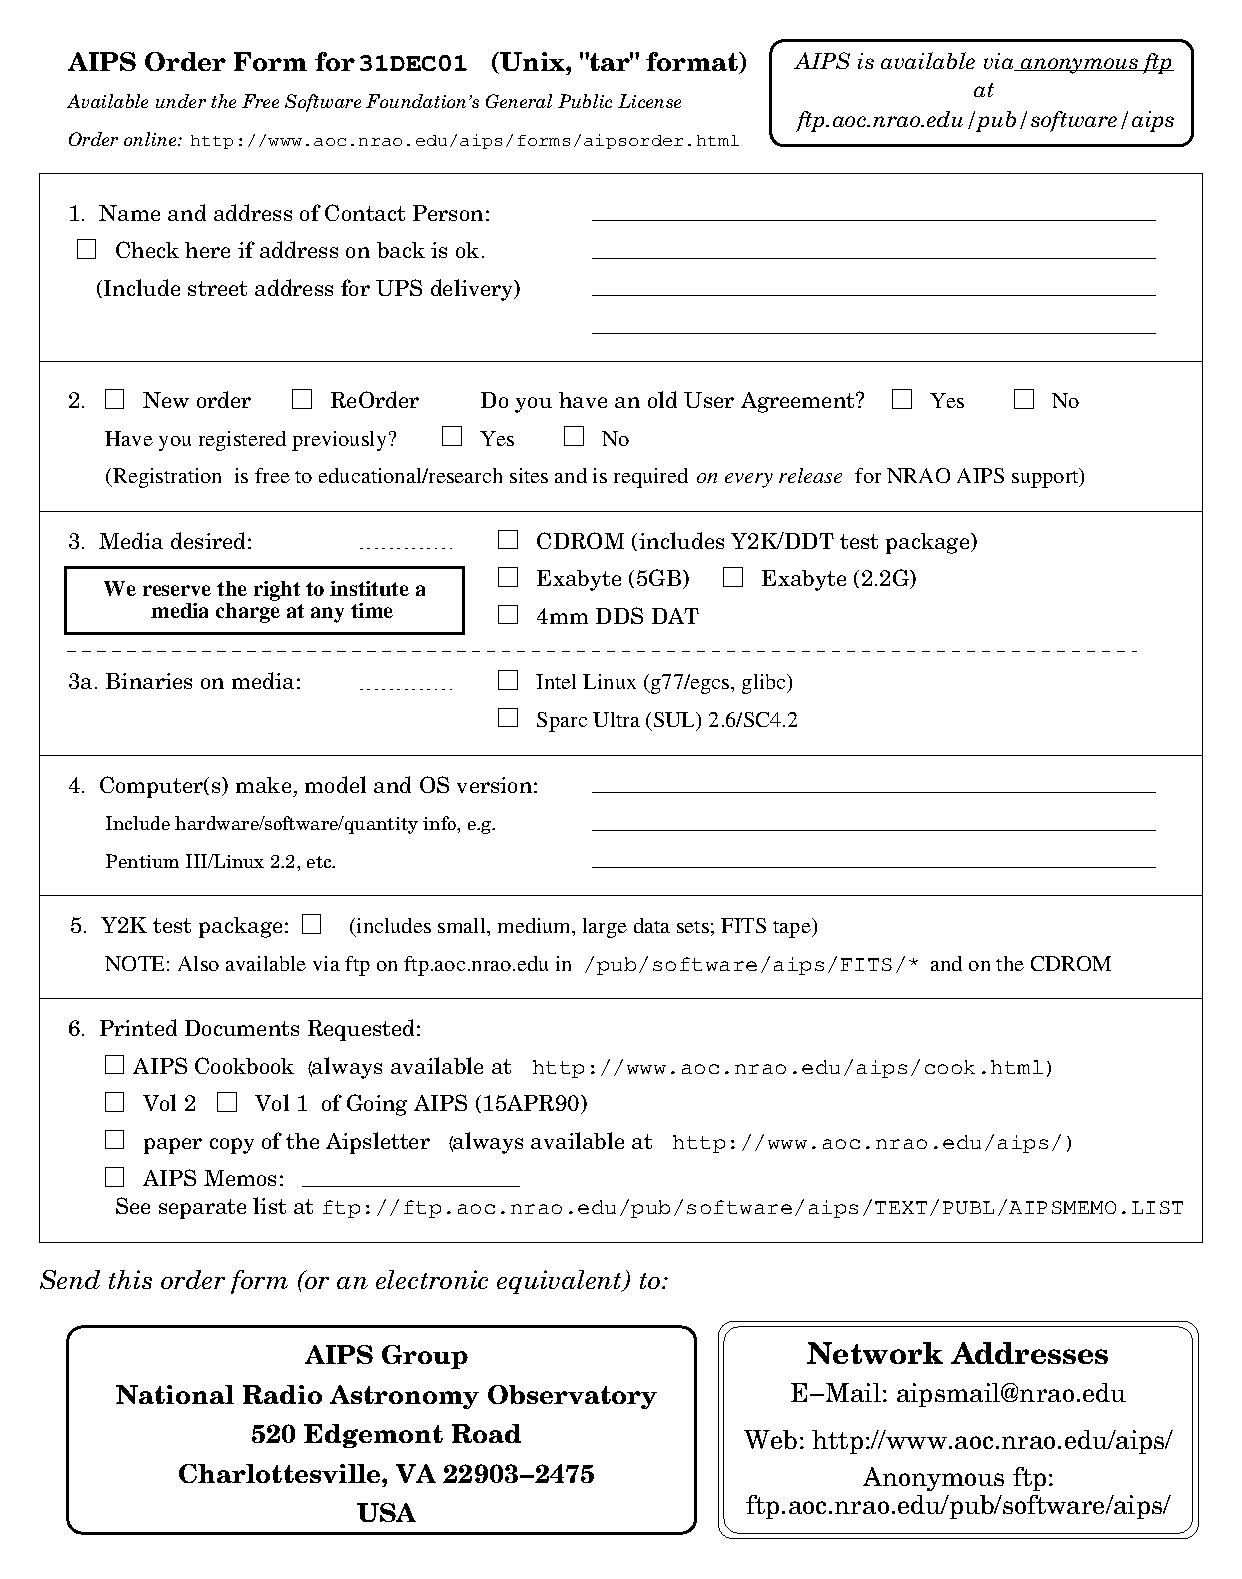
\includegraphics{FIG/AIPSORDER.PS}}}
%\vfill\eject
\vbox to 4.4in{
\vspace{12pt}
\centerline{\rotatebox{-90}{\resizebox{!}{3.5in}{%
\includegraphics{FIG/Mandrill.color.plt}}}}
\vspace{12pt}
\centerline{{\huge \tt \AIPRELEASE}}
\vspace{12pt}
\vfill}
\phantom{...}
\centerline{\resizebox{!}{!}{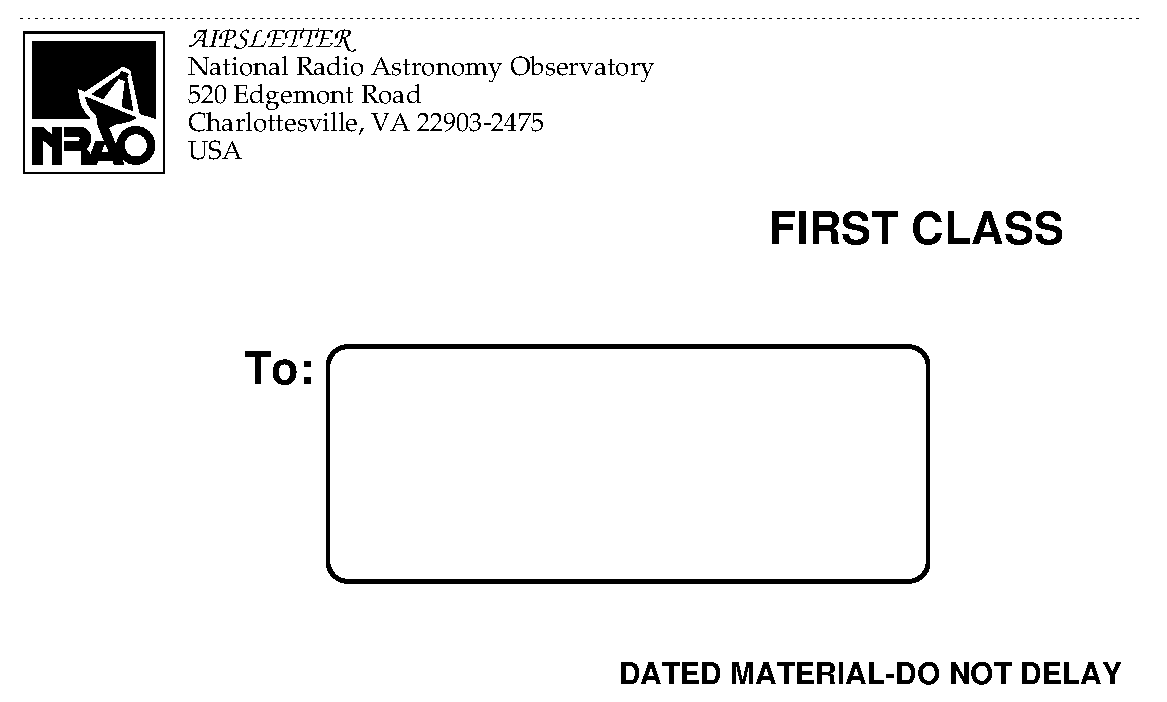
\includegraphics{FIG/AIPSLETM.PS}}}

\end{document}
